%******************************************************************
%******************************************************************
\chapter {Computational Framework}
\label{software}
%******************************************************************
%******************************************************************

In this chapter we describe our computational framework. First, we present the software architecture which is implemented as a modular approach. Then we describe main responsibilities of individual components of each module.
The second part is devoted to high performance computing. First, we show a number of efficient numerical techniques to speed up the computation process. Then we present an implementation of optical flow methods on graphical processing units (GPUs), which enables us to process large datasets in a reasonable time. In the last part of the chapter we describe visualization methods which are implemented in our data analysis framework.


%--------------------------------------------------------
\section {Software Framework}
\label{software_framework}
%--------------------------------------------------------

The software for optical flow computation and time-resolved data analysis is implemented using C++ programming language, is modular and follows the object-oriented design paradigm. The requirements for our implementation are high performance, platform independence and strict control for types and memory management.
Most of the components are implemented within a single unified framework, if not stated otherwise (e.g. some data analysis or data visualization packages are implemented as external routines). In the following section we describe all the software components in more details.


\subsection {Modules}

Our optical flow computation and data analysis framework is designed as a modular system. Each module is responsible for a specific class of functionality. A central part of the framework is a \texttt{CORE} module, which contains classes and methods to perform the optical flow computation. The integral class of this  module is a \texttt{Runner} class which serves as unifying interface and control routine between the core classes and external modules. 
With such organisational architecture it is possible to minimize interdependence between different parts. It also allows to simplify easily the extension or modification of the existing functionality.
The overall diagram of our framework is presented in Figure \ref{fig:software_scheme}.

\begin{figure}[h]
	\centering
	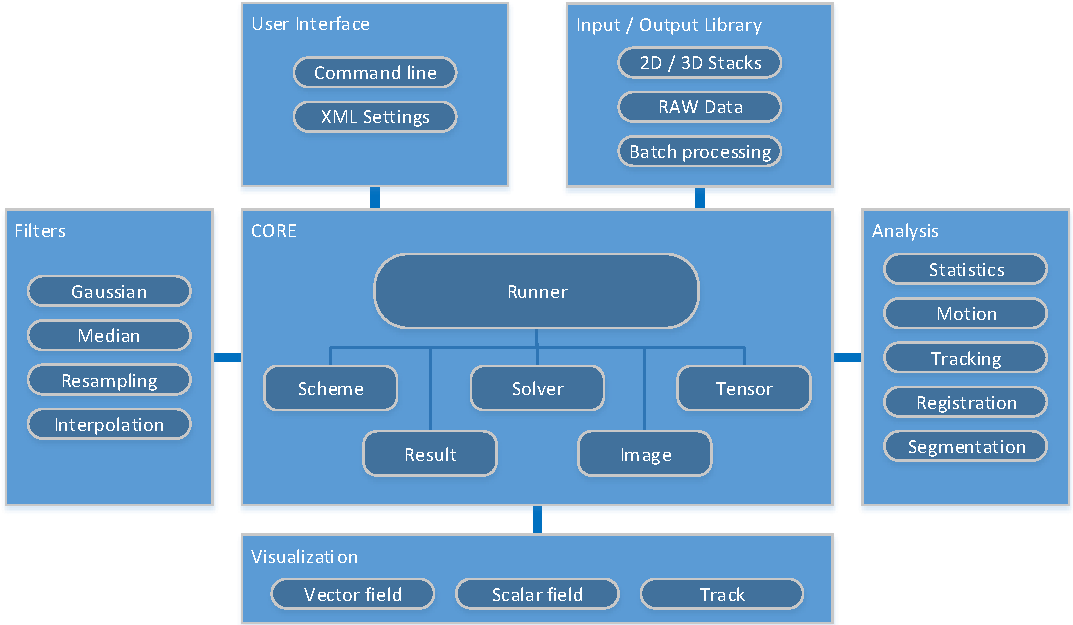
\includegraphics[scale=0.87]{figures/software_scheme.pdf}
	\caption{Optical flow computation and data analysis framework as a modular system. Each model is responsible for a specific class of functionally.  All modules are connected and controlled via the \texttt{Runner} class of the \texttt{CORE} module.}
	\label{fig:software_scheme}
\end{figure}

The developed software framework consists of the following modules:
\begin{itemize}
	\item User interface
	\item Input / Output Library
	\item Filters
	\item Core
	\item Analysis
	\item Visualization	
\end{itemize}

In the following part we describe the responsibility and essential functionality of each of these modules.
\\
\\
\textit{User Interface Module}. Provides an universal interface to setup and adjust the overall workflow, select optical flow models, adjust computation parameters, as well as perform further analysis of the optical flow results. It is implemented as a command line utility and a settings file in a easy-to-read XML format\footnote{\url{http://www.w3.org/XML/}}. 
\\
\\
\textit{Input / Output Library Module}. The module provides routines for data input and output. This includes the work with settings files, statistics, image data, resulting vector fields and other related information. The library allows to use the following data inputs:
\begin{itemize}
	\item 2D / 3D image sequences using common image formats.
	\item RAW data. Using various data types: 8-bit, 16-bit, 32-bit. 
	\item Batch processing. Allows to perform batch processing of long image sequences. Several input modes are possible: masking mode with the specified image indexes; a list of images; a list of image pairs. 
\end{itemize}

\textit{Filters Module}. The module contains various filter which are used during preprocessing, data analysis or optical flow computation. The list of possible image filters includes:
\begin{itemize}
	\item Gaussian smoothing. Implements image filtering via convolution with a Gaussian function  (See Section \ref{noise_filters}).
	\item Median filtering. Implements image filtering using a median filter (See Section \ref{noise_filters}).
	\item Image resampling. Using a number of methods: Averaging, Area-based resampling.
	\item Image interpolation. Available modes: nearest-neighbor, bilinear, trilinear, bicubic interpolations \cite{Parker83}. 
\end{itemize}

\textit{Core Module}.  This module is the central part of the framework and contains classes and methods to perform the optical flow computation, as well as to connect and control the classes from external modules. 
\begin{itemize}
	\item Image. Provides functionality to represent an image in various formats and dimensions. The implemented types of images are: \texttt{Image2D} \texttt{Image3D} and \texttt{ImageRGB}.
	\item Scheme. The main class to impose data constancy assumption via the computation of a motion tensor (See Section \ref{data_constancy_assumptions}). 
	\item Tensor. The class stores the entries of a motion tensor for 2D or 3D image data.
	\item Solver. The main class which performs numerical solution of the optical flow problem via solution of linear equations, which describe the minimum of the energy functional.
	\item Result. This class stores the results of optical flow computation and contains methods to analyze them. In our framework two versions of the optical flow results are implemented - \texttt{Result2D} and \texttt{Result3D} - for two-dimensional and three-dimensional cases respectively.  
\end{itemize}

\textit{Analysis Module}. Contains a set of routines for further analysis based on optical flow results. Some functionality implemented within the same framework and some as external tools.
\begin{itemize}
	\item Motion. A set of methods for further analysis of displacement fields. See Section \ref{motion_analysis} for theoretical description and Section \ref{component_motion} for the list of available functionality. 
	\item Tracking. A module for points or objects tracking using the computed displacement fields as a  feature (See Section \ref{tracking_features}). 
	\item Registration. A module for motion-based image registration (See Section \ref{image_registration}).
	\item Segmentation. Module for motion-based segmentation of moving objects. Thresholding methods are implemented as part of our framework, more advanced methods such as region-growing and level sets methods are implemented externally using Fiji / ImageJ software\footnote{\url{http://imagej.net}}. 
\end{itemize}




\subsection {Components}

%\subsubsection {Hierarchy of Software Components}
%
%\todo{Make figure: All components, interaction}

\subsubsection {Scheme Components}

Scheme components intend to perform the construction of a data term by computation of the corresponding motion tensor (See Section \ref{data_constancy_assumptions}).
A list of available data constancy assumptions implemented as separate \texttt{Scheme} classes includes:
\begin{itemize}
	\item \texttt{Scheme}\texttt{[DataConstancy]}. Performs a computation of a motion tensor for a given constancy assumption. The complete list of available constancy constraint is presented in Section \ref{data_constancy_assumptions}. The implemented constancy modes are \texttt{DataConstancy} = \{\texttt{Grey}, \texttt{Gradient}, \texttt{GreyGradient}, \texttt{GradientNorm}, \texttt{Laplacian}, \texttt{LogDerivatives}, \texttt{GreyRGB}, \texttt{GradientRGB}\}.
	  
	\item \texttt{SchemeNormalization}. All the previously presented data constancy assumptions (list \texttt{DataConstancy}) can be normalized according to the procedure described in Section \ref{normalization}.
	
	\item \texttt{SchemeCLG}. All data assumptions \texttt{DataConstancy} can be convolved with the Gaussian function to obtain a motion tensor which integrates the local information, to obtain the so-called Combined-Local-Global approach (See Section \ref{clg}).
	
	\item \texttt{SchemeMultiChannel}. This scheme allows to construct a data term using an arbitrary number of channels as the input (for example, 3-channel RGB color images). This might be useful to incorporate images obtained using multiple contrast modalities.
	
	\item \texttt{Scheme3D}. All the presented schemes can be implemented for 2D or 3D images. Moreover, implementation for higher dimensions can be extended in a straightforward way.
\end{itemize}


\subsubsection {Solver Components}

The \texttt{Solver} classes perform numerical computation of the optical flow problem, solving a system of  linear equations. Several algorithms are available in our computational  framework (See Section \ref{iterative_methods}): 

\begin{itemize}
\item \texttt{SolverJacobi}. Performs solution of a system of linear equations using a Jacobi method (see Section \ref{jacobi_method}). It is not an optimal solver methods in terms of performance and requires large amount of iteration to converge to the optimal solution. However, for the case of parallel computations, where each element of the matrix is evaluated separately, this solver is more suited (see discussion in Section \ref{jacobi_method}). 

\item \texttt{SolverGauss}. Solves a system of linear equations using a Gau\ss-Seidel method presented in Section \ref{gauss_method}. It speed ups the computation time comparing with the Jacobi methods, since all the entries of the approximation matrix are updated on each iteration. 

\item \texttt{SolverSOR}. Performs the solution using a Gau\ss-Seidel method with the successive overrelaxation technique, which is presented in the section dedicated to the advanced numerical techniques (see Section \ref{sor_method}).

\item \texttt{SolverMultiLevel}. This solver implements a multi-level computation as described in Section \ref{multilevel} and allows to perform high accuracy optical flow computation of large displacements. On each individual computation level the \texttt{SolverJacobi}, the \texttt{SolverGauss} or \texttt{SolverSOR} numerical solvers can be used.

\end{itemize}


\subsubsection {Results Components}
\label{components_results}

The responsibility of this module is to store and analyze the results of optical flow computation.
The following measurements are implemented:

\begin{itemize}
	\item \texttt{EndpointError}. This measure is used to compare two vector fields in terms of a distance between two vectors (See Section \ref{endpoint_error}). Presently it is the most popular measure to compare the computed results with a ground truth displacement field.  
	
	\item \texttt{AngularError}. Computes the angular differences between two vectors (See Section \ref{angular_error}).
	
	\item \texttt{DataConstancyError}. Computes a confidence measure based on the data constancy error (See Section \ref{data_constancy_error}).
	
	\item \texttt{EnergyError}. Computes a confidence measure based on the residual energy of the energy functional (See Section \ref{energy_based_measure}).
	
	\item \texttt{UniquenessError}. Computes a confidence measure based on the motion uniqueness criteria (See Section \ref{motion_uniqueness_criteria}).
	
	\item \texttt{ConsistancyError}. Computes a confidence measure based on the constancy between forward and backward flow fields (See Section \ref{forward_backward_check}).
	
	\item \texttt{PredictionError}. Computes a confidence measure based on the optimal prediction principle (See Section \ref{optimal_prediction_principle}).
	
	\item \texttt{ErrorStatistics}. For each of the error or confidence metrics presented above, a complete set of statistical measure is extracted and can be used. These measures include a minimum (\texttt{min}), a maximum (\texttt{max}), a mean (\texttt{avg}) and standard deviation (\texttt{std}). Moreover, for the endpoint error metrics a set of robust statistics measures is also available. They compute the percentage of pixels that have an error measure larger then a certain amount of pixels. In particular, we compute \texttt{R0.5}, \texttt{R1.0}, and \texttt{R2.0} for the endpoint error, which corresponds to half, one and two pixels error respectively.  
	
	\item \texttt{ErrorRegions}. For every error or confidence metric it is possible to evaluate their statistics in various image regions to get insights how optical flow methods perform in these regions. We provide the following regions of interest: whole image (\texttt{All}), around motion discontinuities (\texttt{Disc}), in textureless regions (\texttt{Untext}), around data artifacts (\texttt{Err}) or in an arbitrary region (\texttt{Roi}). All the regions of interest have to be supplemented to the results analysis routine as binary masks.
	
\end{itemize}

\subsubsection {Motion Analysis Components}
\label{component_motion}

These routines allow to perform further analysis of the computed motion field. The following methods are implemented within our analysis framework:
\begin{itemize}
	\item \texttt{Magnitude}.  See Section \ref{magnitude}.
	
	\item \texttt{Phase}. See Section \ref{phase}.
	
	\item \texttt{Curl}. See Section \ref{curl}.
	
	\item \texttt{Divergence}. See Section \ref{divergence}.
	
	\item \texttt{Components}. The module allows to save individual components of the computed flow field for further analysis.
	
	\item \texttt{Kinematics}.  Allows to extract kinematics components from a motion field. Under assumption of a rigid motion this computational module requires as an input a set of landmarks representing the object of interest, a center of coordinates and an axis of rotation. As an output the component produces a translational (\texttt{trans}) and rotational components (\texttt{rot}) of the object's motion. An example of such motion analysis is presented in Section \ref{app_kinematics_insects}.  
\end{itemize}


\subsubsection {Tracking Components}

These components perform object tracking or tracking of individual points using the results of optical flow computation. With the help of these routine it is possible to perform the following tracking operations:
\begin{itemize}
	\item \texttt{Tracks}. The tracking component takes as an input a set of initial points (landmarks) and performs the tracking procedure using the results of optical flow throughout an image sequence, specified by a number of frames. As an output a list of points and their coordinates on each time frame is produced. A possibility to filter the resulting tracks according to confidence measures, e.g. a consistency measure (See Section  \ref{components_results}), or according to the total distance is also available. An example of this tracking procedure is presented in Section \ref{app_kinematics_insects}. 
	
	\item \texttt{TracksAmira}. The same as the previous methods, but saves the output in a format compatible with the Amira/Avizo software\footnote{\url{http://www.fei.com/}}.
	
	\item \texttt{TracksVTK}. The same as the previous methods, but saves the output in a Visualization Toolkit (VTK) format\footnote{\url{http://www.vtk.org/}}. 
\end{itemize}


%\subsubsection {Temporal Changes Components}













%--------------------------------------------------------
\section {High Performance Computing}
\label{performance}
%--------------------------------------------------------

In this section we discuss such an important aspect as high performance computing. Since optical flow methods are very computationally demanding, an efficient implementation of these techniques should be provided to guarantee that the data processing on a given computational platform is feasible.

First, we discuss several numerical techniques, which allow to speed up the computation time. Then we focus our attention on the implementation of optical flow methods on the GPU architecture.


\subsection{Numerical Schemes}
\label{advanced_numerics}

\subsubsection{Successive-Overrelaxation}
\label{sor_method}

The convergence speed of the Gau\ss - Seidel method can be substantially improved by performing \textit{Successive Overrelaxation} (SOR) technique \cite{Yo71, Saad03}. This is done via extrapolation of the Gau\ss-Seidel result. If we denote by $\bar{\textbf{x}}$ the result of Gau\ss - Seidel method for the iteration step $k+1$, the SOR technique then given by:
$$ \textbf{x}^{k+1}_i = (1-w) \textbf{x}^k_i + w \: \bar{\textbf{x}}^{k+1}_i ,$$
where $w \in [0,2)$ is a \textit{relaxation} parameter.  
Then, The Gau\ss-Seidel method can be extended by the overrelaxation technique in the following way:
$$ x^{k+1}_i = (1-w) x^k_i + w \frac{1}{a_{i,i}} (b_i - \sum_{j < i} a_{i,j} x^{k+1}_j - \sum_{j > i} a_{i,j} x^{k}_j) $$
For the value of relaxation parameter $w=1$, the SOR method comes down to the original Gau\ss-Seidel method. The choice of the relaxation parameter has a strong influence on the convergence speed. A parameter $w$ smaller then 1.0 allows to perform underrelaxation which could lead to improved stability of the algorithm. For the values larger then 1.0 the method performs overrelaxation of the result and thus accelerate the convergence. An optimal value of the relaxation parameter should be chosen according the the specific task. For our applications we select values which are close to the maximum value, such as $w \in [1.9..1.95]$.
A major drawback of the method is a possible oversmoothning of the resulting displacement fields. 


\subsubsection{Adaptive multi-level strategy}

An interesting approach to decrease the computation time is to reduce the input on each computation level. For this purpose the computed flow field is evaluated according to a special criteria. For example one may use the fact that the flow field id varying slowly form one computation level to another. This may highlight that the correct flow has already been estimated. In such regions the computationally expensive energy minimization is substituted by a simple interpolation from the results of previous computation levels. Such approach was presented by the authors in \cite{CGF3013} and allowed to significantly reduce the computation time without serious impact on the accuracy of the overall result. This approach can be especially advantageous for datasets with small or isolated objects and dominance of the static background. In this cases an adaptive computation procedure removes most of the irrelevant computations in the background region.    


%\subsubsection{Combining Different Algorithms}
%
%\todo{Give reference to Fusion Flow paper}
%\comment{Add information about combination of efficient and fast implementation with a successive run of high precision OF implementation . From \cite{CGF3013} Show references}
%



\subsection{GPU Computing}   
\label{gpu} 


This section is dedicated to a GPU-based implementation of the optical flow algorithm. First, we briefly discuss the key features of the GPU architecture \cite{nvidiatoolkit, nvidia2010developer}. Then we introduce a GPU-based implementation that uses only one GPU device and is limited to the datasets that can be fitted in the GPU memory. The main aspects of the implementation are discussed in details. Finally, we show how a single GPU device version can be extended in order to process arbitrary large datasets.


%--------------------------------------------------------
\subsubsection{GPU Computing Architecture}
%--------------------------------------------------------
For the GPU implementation of 3D optical flow methods we choose a NVIDIA CUDA technology\footnote{\url{http://www.nvidia.com/object/cuda_home_new.html}}. However, all finding presented in the current section are valid or can be implemented by means of other GPU platforms, for example, OpenCL\footnote{\url{https://www.khronos.org/opencl/}}.
\\
\\
\textbf{Host-device execution model}
\\
\\
In general a GPU computing architecture is comprised of two essential parts - a \textit{host} and a \textit{device} \cite{nvidiatoolkit}. Alternative notation is a CPU for the host and a GPU for the device. The host manages the device by scheduling control commands and sending them to the device. The code execution on the host and the device can be done \textit{synchronously} or \textit{asynchronously}. For the case of synchronous execution mode, the host waits until a command is completed on the device and only after the continues to execute its pipeline. If the control commands are scheduled in an asynchronous mode, the host receives the control immediately after sending a command to the device. Such mechanism implements a strategy, for which the host and the device can perform different tasks simultaneously. All the commands sent by the host are queued for sequential execution on the device side. In terminology of CUDA such queues are called \textit{streams}. All the commands are executed in issue-order and there is no possibility to run several commands within the same stream. However, a single device has many processing streams which can be executed in parallel. 
\\
\\
\textbf{Device execution model}
\\
\\
The commands to be send from the host to the device can be memory management commands, such as memory allocation, deallocation or copy, and also control synchronization or profiling commands. Additionally, the host can send a special command to launch a \textit{kernel} on the device. Kernels are the core elements of the GPU computing.  A kernel is a user-defined function which can be run on the device. All the kernel's instructions are executed sequentially, while multiple copies of such kernels are run in parallel on the device. The kernel code is written in the CUDA C-based language and then compiled into a binary code for the specific GPU device \cite{nvidiatoolkit}.

Multiple kernels are organized in \textit{thread blocks}, which in turn make a grid of thread blocks. Both threads and thread blocks have unique indexes.  Thread blocks and a grids can be organized as one-, two- or three-dimensional structures.  Only a limited amount of thread can be run on a single GPU multi-processor. It is important to note, that the execution order of thread blocks and each thread within a block is not guaranteed.  
\\
\\
\textbf{Memory model}
\\
\\
In the GPU computing the memory model is divided into a host memory (system memory) and device memory (GPU memory).
Both parts have the direct access only to its own memory resources.  

There are several distinct types of GPU memory:
\begin{itemize}
	\item \textbf{Device memory} is a global memory shared between all streaming multi-processors. The access to the device memory has highest access latency, and therefore it is the slowest type of memory. The device memory can be accessed by all threads. Moreover, it can be accessed from the host by using memory management functions. The aim of many optimization strategies is to minimize the amount of memory accesses to the global memory and reduce the data transfer between the host and the device.  
	
	\item \textbf{Texture memory} is optimized for storing and accessing textures. This type of device memory is read-only.
	Using this memory one can benefit from the built-in hardware functionality (e.g. interpolation).
	
	\item \textbf{Constant memory} allows to store limited amount of constant data.
	
	\item \textbf{Shared memory} serves as a low latency storage accessible from all threads within an individual block. 
	
	\item \textbf{Registers} memory belong to the fastest GPU memory type. Each streaming multi-processor has a limited amount of registers which are shared between all threads within a thread block. Registers are used to store local variables of a single thread. 
\end{itemize}

Clearly, each type of GPU memory has its pros and cons. To achieve maximum performance we have to efficiently use all types of GPU memory and adjust the implementation of the GPU-based parallel algorithm accordingly.

\subsubsection{GPU implementation}


To maximize the performance of GPU-based optical flow algorithm, we provide a first GPU implementation, a \textit{full} GPU version. In this version all data is stored in the GPU memory. In this way the data transfer between the host and the device is minimized. Cleary a limitation factor for this kind of implementation is the size of available GPU memory. Now, we estimate the size of input frames which is possible to process using such GPU method. For a 3D image with $width \times height \times depth$ voxels, assuming that each voxel is represented by a single-precision floating-point number, the size of such a 3D image is then equals to $width \times height \times depth \times 4$ bytes. To solve the optical flow problem we need 2 such volumes. Additionally, we need containers for the vector field results, each having 3 flow components $u$, $v$ and $w$. Moreover, we need  auxiliary containers to store intermediate results of the optical flow algorithm. In total we need to allocate 15 single-precision floating-point containers with the size $width \times height \times depth \times 4$. Figure \ref{fig:data-copy} gives a schematic overview of allocated data and the data transfer procedure.  

\begin{figure}[h]
	\centering
	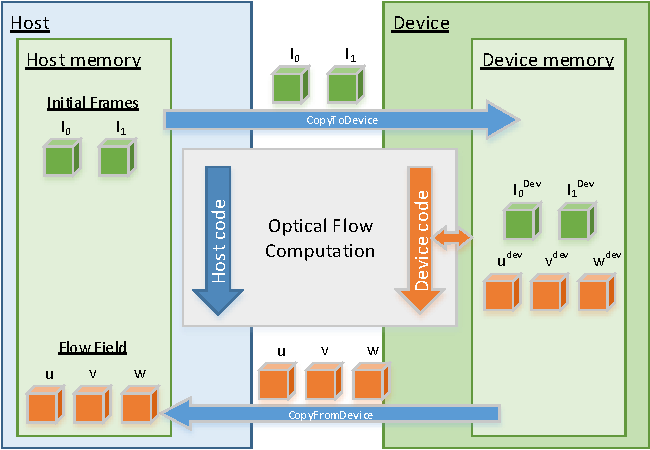
\includegraphics[width=.65\textwidth]{figures/data-copy.pdf}
	\caption{Data transfer between the host and the device for the GPU based implementation of the 3D optical flow algorithm. Image: \cite{KarlinskiyThesis}.}
	\label{fig:data-copy}
\end{figure}

Then, we can estimate the maximum size of the input frame which is possible to process using full GPU version: 
\begin{equation}
15 \times pitch \times height \times depth \times sizeof(float) \leq N.
\end{equation}  
As an example, if we have a GPU with 4GB of memory, we can process input volumes of approximately 273MB, which corresponds to a volume with the sizes about $400 \times 400 \times 400$ voxels.
Obviously, such data sizes are not adequate, if we consider the processing of high-resolution datasets. For large datasets it is then necessary to downsample the initial data, which could lead to a significant loss in resolution and accuracy. To overcome this limitation and enable the processing of large datasets in the next section we present an extension of our GPU implementation.

\subsubsection{Extension for large datasets}

In this section we show how the 3D optical flow method can be extended to support large datasets.
The main idea of the proposed method is to implement the so-called \textit{data partitioning strategy}. We store the dataset and corresponding vector fields in the host memory and transfer smaller portions to the device for parallel processing on GPU. In this strategy, the host performs managing of the data partitioning, execution on the device and collection of the results after each computation level. To perform data partitioning we make the slicing of the original volumes and extend each data chunk with overlapping regions, solve the data dependency problem.   
An example of such partitioning (slicing along Z-axis) is presented in Figure \ref{fig:slicing-overlap}.

\begin{figure}[h]
	\centering
	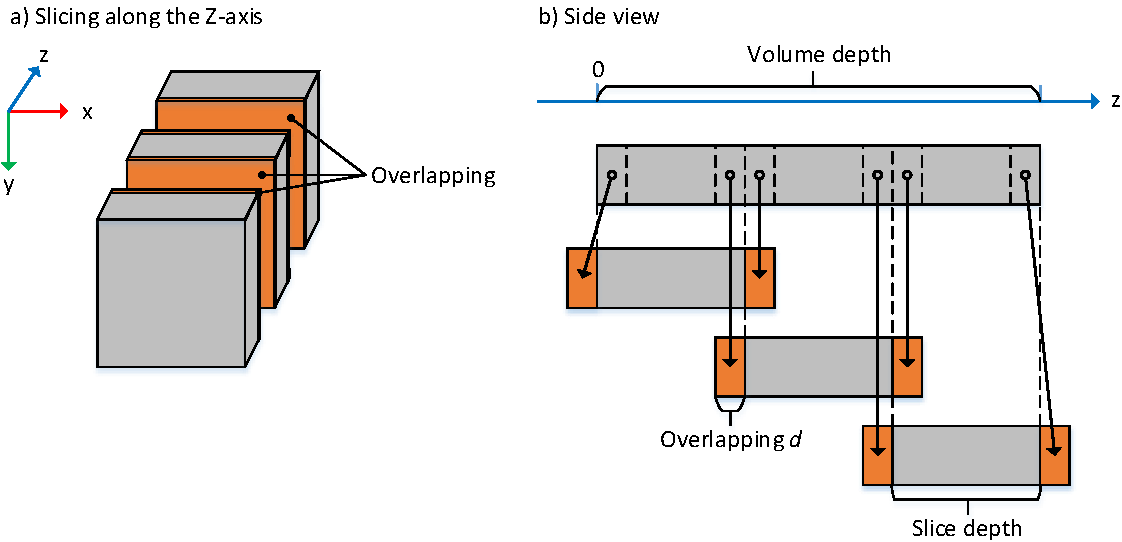
\includegraphics[width=0.8\textwidth]{figures/slicing-overlap.pdf}
	\caption{Data partitioning strategy. Slicing is done along the Z-axis with the overlapping regions (a). Partitioning of voxels in the full volume with overlapping regions (b). The overlapping regions that are outside the full volume are filled with "mirrored" values. Image: \cite{KarlinskiyThesis}.}
	\label{fig:slicing-overlap}
\end{figure}

Note, that in the previous implementation (\textit{full} GPU version) the whole dataset, the resulting vector fields and all auxiliary containers reside in the GPU memory and there is only one data transfer operation from the host to the GPU. In our \textit{extended} version data is transferred between the host and the device before and after processing of each data chunk. Therefore, data transfer can lead to serious performance issues and the bandwidth between the host and the device become a limiting factor. In the next section we provide quantitative performance analysis between CPU and GPU versions, as well as between \textit{full} and \textit{extended} GPU versions.


\subsubsection{Performance evaluation}

To measure the performance of our GPU based 3D optical flow implementation we run the method on datasets with different sizes. Instead of evaluating each individual component of the algorithm, we present the execution time and memory consumption for the whole computation pipeline. Moreover, we verify the correctness of the algorithms compared with the original CPU implementation.   

For the evaluation we use the computation hardware with the specifications presented in Table \ref{tbl:test-machines}.

\begin{table}[h] \scriptsize
	\centering
	\begin{tabular}{l c c}
		\hline
		& CPU Test machine           & GPU Test machine                                                                                  \\
		
		\hline
		CPU        & Intel Xeon Processor X5675 & Intel Xeon Processor E5-2637 v2                                                                   \\
		RAM        & 96 GB                      & 64 GB                                                                                             \\
		GPU        & ---                        & GeForce GTX 980 Ti
		 \\
		GPU Memory & ---                        & 6 GB                                                                                              \\
		CUDA Cores & ---                        & 2816                                                                                             
	\end{tabular}
	\caption{Technical specifications of computation machines used for the performance evaluation.}
	\label{tbl:test-machines}
\end{table}

We estimate how the size of the input data influences performance of 3D optical flow method and the memory consumption by the computation routines. For the evaluation we use  datasets with the following sizes: $100^3$, $200^3$, $400^3$, $600^3$, $800^3$. As it was highlighted previously for a GPU device with 4GB of memory the maximum size of the input data is $400^3$. Therefore, datasets with sizes $100^3$, $200^3$ and $400^3$ can be processed using \textit{full} GPU method; while larger dataset - $600^3$, $800^3$, can be processed only using an \textit{extended} version. 
Evaluation results for performance measurements and memory consumption are presented in Tables \ref{tb:perf-time} and \ref{tb:perf-mem} respectively.

\begin{table}[h] \footnotesize
	\centerline{
		\begin{tabular}{c|c|c|c|cc}
			\multirow{2}{*}{\begin{tabular}[c]{@{}c@{}}Size\\ (voxels)\end{tabular}} & \multicolumn{3}{c|}{\begin{tabular}[c]{@{}c@{}}Execution time\\ (hh:mm:ss)\end{tabular}}                                                                              & \multicolumn{2}{c}{\begin{tabular}[c]{@{}c@{}}Speedup\\ relative to CPU verion\end{tabular}}                                                     \\ \cline{2-6} 
			& \begin{tabular}[c]{@{}c@{}}GPU\\ \textit{Full} version\end{tabular} & \begin{tabular}[c]{@{}c@{}}GPU\\ \textit{Extended} vesion\end{tabular} & \begin{tabular}[c]{@{}c@{}}CPU\\ Version\end{tabular} & \multicolumn{1}{c|}{\begin{tabular}[c]{@{}c@{}}GPU\\ \textit{Full} version\end{tabular}} & \begin{tabular}[c]{@{}c@{}}GPU\\ \textit{Extended} version\end{tabular} \\ \hline
			$100^3$                                                                                 & 00:00:01                                                   & 00:00:13                                                      & 00:00:38                                              & \multicolumn{1}{c|}{41.8}                                                        & 2.9                                                            \\
			$200^3$                                                                                 & 00:00:03                                                   & 00:00:42                                                      & 00:06:02                                              & \multicolumn{1}{c|}{112.4}                                                       & 8.6                                                            \\
			$400^3$                                                                                 & 00:00:19                                                   & 00:03:52                                                      & 01:13:52                                              & \multicolumn{1}{c|}{\textbf{239.4}}                                                       & \textbf{19.1}                                                           \\
			$600^3$                                                                                 & ---                                                        & 00:11:48                                                      & 02:47:53                                              & \multicolumn{1}{c|}{---}                                                        & 14.2                                                            \\
			$800^3$                                                                                 & ---                                                        & 00:26:33                                                      & 07:30:49                                              & \multicolumn{1}{c|}{---}                                                        & 17                                                           
		\end{tabular}
	}
	\caption{Evaluation of execution time for dataset with different sizes $100^3$, $200^3$, $400^3$, $600^3$, $800^3$.}
	\label{tb:perf-time}
\end{table}

\begin{table}[h] \footnotesize
	\centering
	\begin{tabular}{c|c|c|cc}
		\multirow{2}{*}{\begin{tabular}[c]{@{}c@{}}Size\\ (voxels)\end{tabular}} & \multicolumn{2}{c|}{\begin{tabular}[c]{@{}c@{}}GPU\\ \textit{Full} version\end{tabular}} & \multicolumn{2}{c}{\begin{tabular}[c]{@{}c@{}}GPU\\ \textit{Extended} version\end{tabular}} \\ \cline{2-5} 
		& Device memory                          & System memory                          & \multicolumn{1}{c|}{Device memory}                 & System memory                 \\ \hline
		$100^3$                                                                                 & 73 MB                                  & 19 MB                                  & \multicolumn{1}{c|}{*}                           & 57 MB                         \\
		$200^3$                                                                                 & 586 MB                                 & 153 MB                                 & \multicolumn{1}{c|}{*}                           & 458 MB                        \\
		$400^3$                                                                                 & 3.64 GB                                & 1.19 GB                                & \multicolumn{1}{c|}{*}                           & 3.58 GB                       \\
		$600^3$                                                                                 & ---                                    & ---                                    & \multicolumn{1}{c|}{*}                           & 12.07 GB                      \\
		$800^3$                                                                                 & ---                                    & ---                                    & \multicolumn{1}{c|}{*}                           & 28.61 GB                     
	\end{tabular}
	\caption{Memory usage of the implemented framework. Note that the memory allocated on the device is padded to satisfy alignment requirements. (*) For the extended version the usage of the device memory is determined by the current needs for the sliced data and available GPU memory.}
	\label{tb:perf-mem}	
\end{table}

From time measurements we see the following results - for small datasets $\le 400^3$), \textit{full} GPU implementation gives the best performance. Clearly, the \textit{extended} version provides less performance compared to the \textit{full} version due to data transfer operations between the host and the device. However, for larger datasets ($> 400^3$), the \textit{full} version is no longer functional, since the data cannot be fitted into the memory of the GPU, so the data partitioning strategy of the \textit{extended} version has to be used. In this case, the \textit{extended} version significantly outperforms the CPU version of the optical flow method. The maximal performance speedup for the \textit{full} version was 33.5, for the \textit{extended} version -- 11.5. Therefore, we conclude that our 3D GPU-based implementation is efficient and provides a significant reduction in the computation time for large 3D datasets.




%--------------------------------------------------------
\section {Visualization}
%--------------------------------------------------------
\label{visualization}

The section gives a brief summary of visualization methods for time-varying data and results of optical flow computation which are available in our data analysis framework. We implement three main visualization methods:
\begin{itemize}
	\item Vectors fields using glyphs visualization 
	
	\item Scalar properties or other metrics using color pseudo-codes.
	
	\item Motion trajectories using track visualization 
\end{itemize} 

In the following part we describe in more details vector fields visualization using vector glyphs and omit the description of other methods. 

%Examples of vector field visualization and scalar field visualization using magnitude are shown in Figure \ref{fig:vis_vec_comp} alongside with the correspond 3D rendering.
%
%\begin{figure*}[t]
%	\centerline{
%		\mbox{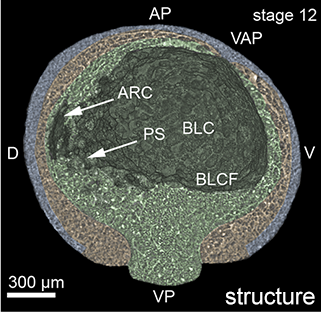
\includegraphics[scale=0.85]{figures/vis_vec_comparison1.png}}
%		\mbox{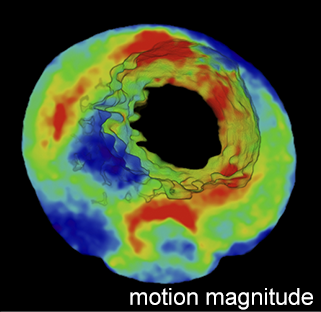
\includegraphics[scale=0.85]{figures/vis_vec_comparison2.png}}
%	}
%	\caption[]{\textbf{Left:} 3D rendering of a halved embryo. \textbf{Right:} 3D rendering of a scalar field representing velocity magnitude.}
%	\label{fig:vis_vec_comp}
%\end{figure*}


\subsection*{Vector Field}

A simple yet effective method for visualization of vectors fields is a glyphs method. In this case each vector of the displacement field is depicted as a glyph with a certain shape and color. 

For our implementation we use 3D cones. For the coloring of glyphs we use two modes: the first one assigns a color according to the magnitude of a vector and the second mode uses the direction of a vector. Both visualization using different coloring schemes are presented in Figure \ref{fig:vec_vis}.

\newcommand{\imageSizex}{0.29}

\begin{figure}[ht]
	\centerline{	
		\mbox{\includegraphicslabeledb[scale=\imageSizex]{figures/magnitude.png}{a}}	
		\mbox{\includegraphicslabeledb[scale=\imageSizex]{figures/direction.png}{b}}
	}	
	\centerline{	
			\mbox{\includegraphicslabeledb[scale=\imageSizex]{figures/threshold-1.png}{c}}	
			\mbox{\includegraphicslabeledb[scale=\imageSizex]{figures/threshold-0.png}{d}}
    }    	
   	\centerline{	
   		\mbox{\includegraphicslabeledb[scale=\imageSizex]{figures/regular.png}{e}}	
   		\mbox{\includegraphicslabeledb[scale=\imageSizex]{figures/jittered.png}{f}}
   	}
		
	\caption{Visualization of a 3D vector field. \textbf{(a)} Using magnitude of the vectors for coloring.  \textbf{(b)}  Using direction of the vectors for coloring.  \textbf{(c)} Regular grid, no threshold of magnitude value. \textbf{(d)} Regular grid, threshold is applied. \textbf{(e)} Regular grid, decreased number of grid points. \textbf{(f)} Jittered grid. Image adopted from: \cite{KarlinskiyThesis}.}
	\label{fig:vec_vis}
\end{figure}

In order to improve the usability of the 3D visualization tool we provide visualization parameters that can be changed interactively. It is possible to adjust the sample grid $G_x$, $G_y$, $G_z$, the glyphs scaling factor and the magnitude threshold. All different visualization modes are presented in Figure \ref{fig:vec_vis}. Moreover, it is possible to use the so-called \textit{jittered} grid. It allows to avoid possible artifacts associated with the regular grid (artifacts similar to aliasing, when viewed from different angles). This improves the clarity of user’s perception of different parts of the vector field. Comparison between a regular and a jittered grid is given in Figure \ref{fig:vec_vis}. All the visualization parameters can be adjusted interactively and the changes are immediately rendered.




%\begin{figure}[h]
%	\centerline{
%		\mbox{\includegraphicslabeledb[scale=0.27]{figures/threshold-1.png}{a}}
%		\mbox{\includegraphicslabeledb[scale=0.27]{figures/threshold-0.png}{b}}
%	}
%	\caption{Different visualization modes. \textbf{(a)} Regular grid, no threshold of magnitude value. \textbf{(b)} Regular grid, threshold is applied. Image: \cite{KarlinskiyThesis}.}
%	\label{fig:vis_modes}
%\end{figure}

%\begin{figure}[h]
%	\centerline{
%		\mbox{\includegraphicslabeledb[scale=0.27]{figures/regular.png}{a}}
%		\mbox{\includegraphicslabeledb[scale=0.27]{figures/jittered.png}{b}}
%	}
%	\caption{Different visualization modes. \textbf{(a)} Regular grid, decreased number of grid points. \textbf{(b)} Jittered grid. Image: \cite{KarlinskiyThesis}.}
%	\label{fig:vis_modes2}
%\end{figure}

For the implementation of our visualization tool we use OpenGL\footnote{\url{https://www.opengl.org/}} as a 3D graphics library, GLFW\footnote{\url{http://www.glfw.org/}} as a library for window and input management, GLM\footnote{\url{http://glm.g-truc.net/}} as a mathematics library for graphics software and AntTweakBar\footnote{\url{http://anttweakbar.sourceforge.net/}} as a light graphical user interface library. All the libraries are cross-platform and free to use.

        
%\subsection{Scalar Field}
%For visualization of scalar fields (see the whole list of metrics in Sections \ref{components_results} and \ref{component_motion}) in 2D or 3D we use a number of look-up tables (LUTs).
%\todo{change: From. Russ.}\change{The use of color scales as a substitute for brightness values allows us to show and see small
%changes locally, and identify the same brightness values globally in an image. This should be
%a great benefit, since these are among the goals for imaging discussed below. Color might be used  to encode flow components, velocity, differently moving objects and other quantitative.
%These uses generally have little to do with the properties of the image and simply take advantage
%of the human ability to distinguish more colors than grey scale values.}
%For visualization of scaler fields we use external software such as ImageJ / Fiji.
%An example of color coding using different LUTs is given in Figure \ref{fig:lookup_tables}.
%
%\begin{figure*}[!ht]
%  \centerline{
%    \mbox{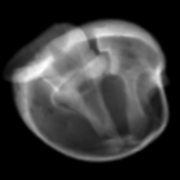
\includegraphics[scale= 0.6]{figures/lut_screw_grey.png}}
%    \mbox{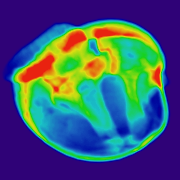
\includegraphics[scale= 0.6]{figures/lut_screw_physics.png}}
%    \mbox{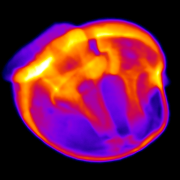
\includegraphics[scale= 0.6]{figures/lut_screw_fire.png}}
%  } 
%  \vspace{3pt}
%   \centerline{
%    	\mbox{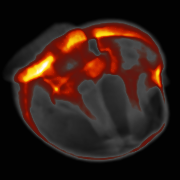
\includegraphics[scale= 0.6]{figures/lut_screw_smart.png}}
%    	\mbox{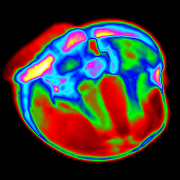
\includegraphics[scale= 0.6]{figures/lut_screw_6_shades.png}}
%    	\mbox{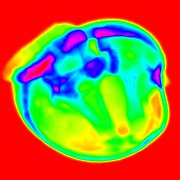
\includegraphics[scale= 0.6]{figures/lut_screw_spectrum.png}}
%    }
%
%  \caption[Noise filterst]{Color coding of a projection radiograph using different color-codes. Note that different local and global image features are highlighted by each look-up table.}
%  \label{fig:lookup_tables}
%\end{figure*}




%\subsection{Line Convolution}
%
%[pages 0.5-1]
%
%\begin{itemize}
%	\item Name
%  \item Description, Shows what?
%  \item Example image
%  \item Best usage examples
%\end{itemize}

%\subsection{Tracks}
%
%Visualization of tracking information is implemented using external software packages such as Amira/Avizo software\footnote{\url{http://www.fei.com/}} and Paraview\footnote{\url{http://www.paraview.org/}}.
%Our computational framework outputs the tracking information in formats, recognizable by these software packages. Few examples of tracks visualization using Avizo software are presented in Figure \ref{fig:vis_vec_comp}. 
%	 
%
%\begin{figure*}[!ht]
%	\centerline{
%		\mbox{\includegraphicslabeledw[scale=0.35]{figures/vis_tracks_random.png}{a}}
%		\mbox{\includegraphicslabeledw[scale=0.35]{figures/vis_tracks_arch.png}{b}}
%	}
%	\caption[]{\todo{Extend description}Visualization example of tracking information.  \textbf{(a)} Short tracks of cells distributed on a regular grid. The color denotes time. \textbf{(b)} Tracking of morphological changes in internal structures. \change{Colors correspond to outlines of different organs.}}
%	\label{fig:vis_vec_comp}
%\end{figure*}





%\subsection{Color Coding}
%
%Link: http://hci.iwr.uni-heidelberg.de/Static/correspondenceVisualization/
%
%To show:
%\begin{itemize}
%	\item 2D Bruhn colors
%	\item 2D Middl colors
%  	\item 3D RGB cube
%  	\item 3D projections: XY, YZ, XZ
%  	\item Simplified colors: 6, more
%\end{itemize}






